The standard Richards function treats hazard intensity as instantaneous: a flood of depth $h$ produces damage ratio $\DF(h)$ regardless of whether the water recedes after two hours or persists for two weeks. This assumption is adequate for acute hazards such as hailstorms but significantly underestimates damage for prolonged flooding, where water contact duration drives additional degradation through material saturation, mould growth, electrical system failure, and structural weakening.

We extend the Richards function by making its parameters depend continuously on hazard duration $\tau$:

\begin{equation}
    \DF(h, \tau) = \frac{1}{\left(1 + Q(\tau) \exp\left[-B \cdot \left(\frac{h - F_{\min}}{F_s - F_{\min}} - a(\tau)\right)\right]\right)^{1/\nu(\tau)}}
    \label{eq: duration richards}
\end{equation}
where the duration-dependent parameters are:
    $a(\tau) = a_0 \cdot \exp\left(-\lambda_a \cdot \frac{\tau}{\tau_0}\right)$,
    $Q(\tau) = Q_0 \cdot \exp\left(-\lambda_Q \cdot \frac{\tau}{\tau_0}\right)$, 
    $\nu(\tau) = \nu_0 + \delta_\nu \cdot \ln\left(1 + \frac{\tau}{\tau_0}\right)$. 

Here $\tau_0 = 48$~hours is a reference duration scale, and $\lambda_a$, $\lambda_Q$, $\delta_\nu$ are duration sensitivity coefficients. The physical interpretation is:
\begin{itemize}
    \item $a(\tau)$ controls the inflection point: as duration increases, the ``50\% damage depth'' shifts toward shallower water, reflecting the empirical observation that prolonged shallow flooding causes damage comparable to brief deep flooding;
    \item $Q(\tau)$ controls onset speed: longer duration accelerates the transition from zero to significant damage;
    \item $\nu(\tau)$ controls curve asymmetry: prolonged events produce concave (fast-onset, slow-saturation) curves rather than the symmetric sigmoid of instantaneous events.
\end{itemize}

At $\tau = 0$, the function reduces exactly to the standard Richards form (Eq.~\ref{eq: logistic function}) with parameters $(B, Q_0, a_0, \nu_0)$, ensuring backward compatibility. The total number of calibratable parameters is seven: $(B, Q_0, a_0, \nu_0, \lambda_a, \lambda_Q, \delta_\nu)$.

The duration-dependent extension produces a continuous family of damage curves that transitions smoothly from a sigmoidal shape (instantaneous events) to a concave form (prolonged events). Fig.~\ref{fig:duration_curves} illustrates the effect: as $\tau$ increases, the inflection point shifts leftward (toward shallower depths), so that even moderate flooding causes substantial damage after prolonged inundation.

\begin{figure}[ht]
\centering
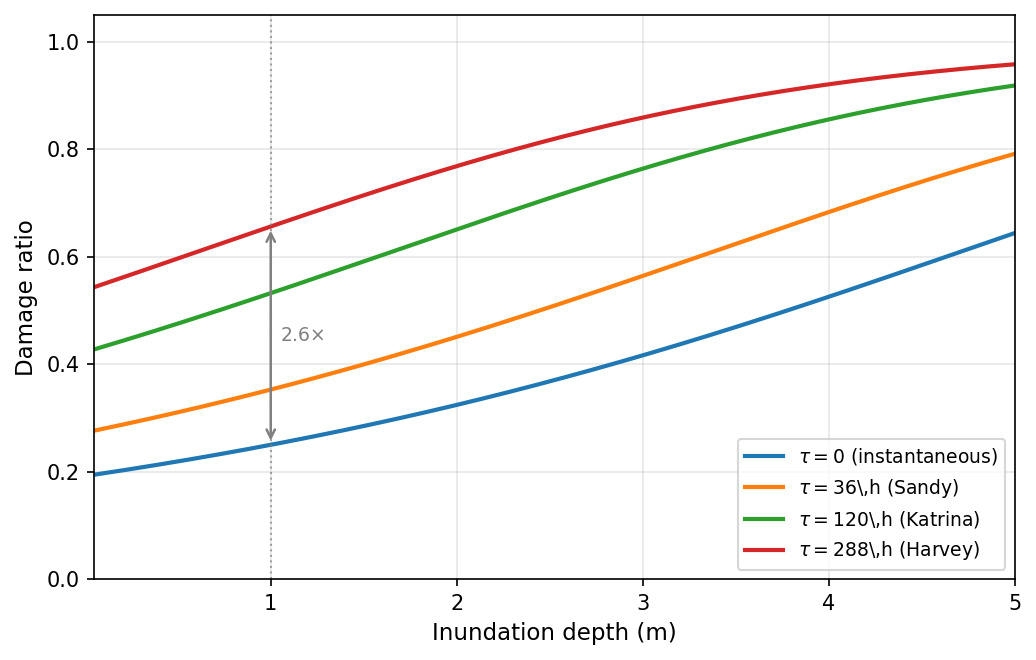
\includegraphics[width=0.75\textwidth]{Content/Images/duration_curves.png}
\caption{Duration-dependent flood damage function: as inundation duration $\tau$ increases, the inflection point shifts toward shallower depths. At 1\,m depth, DF rises from 0.25 (instantaneous) to 0.66 ($\tau = 288$\,h), a 2.6 times amplification. Curves are plotted from $h_{\min} = 0.05$\,m; the Richards function is not defined to start at $h = 0$ because the minimum inundation threshold excludes negligible-depth events.}
\label{fig:duration_curves}
\end{figure}
